\documentclass[11pt]{article}
\usepackage[utf8]{inputenc}
\usepackage{graphicx}
\usepackage{hyperref}
\usepackage{booktabs}
\usepackage{float}
\usepackage{amsmath}
\usepackage{listings}
\usepackage{xcolor}

% Code listing settings for bash scripts
\lstset{
    basicstyle=\ttfamily\small,
    frame=single,
    breaklines=true,
    language=bash
}

\title{ParallelMST: A Parallel Implementation of Minimum Spanning Tree Algorithms Using OpenMP}
\author{Prithviraj Murthy}
\date{\today}

\begin{document}

\maketitle
\tableofcontents
\newpage

\begin{abstract}
This report documents the design, implementation, and performance evaluation of the \textbf{ParallelMST} project. The project features parallel and sequential implementations of two classic MST algorithms (Kruskal's and Prim's) using OpenMP. Multiple sorting methods (Bubble, Quick, and Merge Sort) are employed to compare performance across various graph sizes. This report covers system requirements, build and usage instructions, testing methodologies, and detailed performance evaluations.
\end{abstract}

\section{Introduction}
Minimum Spanning Tree (MST) algorithms are fundamental in solving network design and optimization problems. The \textbf{ParallelMST} project focuses on employing parallel processing techniques via OpenMP to improve the performance of MST computations. In this document, we present our approach, testing scenarios, and detailed performance comparisons between parallel and sequential implementations.

\section{Project Overview}
\subsection{Implemented Algorithms}
The project provides both sequential and parallel implementations of the following MST algorithms:
\begin{itemize}
    \item \textbf{Kruskal's Algorithm}
    \item \textbf{Prim's Algorithm}
\end{itemize}
Each algorithm is implemented with three different sorting methods:
\begin{itemize}
    \item Bubble Sort
    \item Quick Sort
    \item Merge Sort
\end{itemize}

\subsection{Key Features}
\begin{itemize}
    \item Parallel implementations built with OpenMP.
    \item Multiple sorting options available for performance tuning.
    \item Performance comparisons between sequential and parallel implementations.
    \item Utility for graph generation.
\end{itemize}

\section{Background and Algorithm Explanations}
\subsection{Minimum Spanning Tree Algorithms}
In this project, we have implemented two classic MST algorithms:

\paragraph{Prim's Algorithm:} 
Prim's algorithm is a greedy approach that constructs a minimum spanning tree (MST) by starting with an arbitrary vertex and repeatedly adding the smallest edge that connects a vertex in the tree to a vertex outside the tree. This process continues until all vertices are included. Using data structures such as priority queues can improve its performance to approximately $O(E \log V)$ for dense graphs.

\paragraph{Kruskal's Algorithm:} 
Kruskal's algorithm begins by sorting all graph edges in order of increasing weight. It then iteratively adds the next smallest edge to the spanning tree if the edge does not form a cycle, which is efficiently checked using a union-find data structure. The dominant cost of this algorithm comes from the sorting step, giving it a time complexity of $O(E \log E)$.

\subsection{Sorting Algorithms}
Sorting is a crucial component, particularly for Kruskal's algorithm. We implemented three different sorting methods to explore their impact on performance:

\paragraph{Bubble Sort:} 
Bubble Sort is a simple comparison-based algorithm that repeatedly goes through the list, compares adjacent items, and swaps them if they are in the wrong order. Although easy to implement, it has an inefficient time complexity of $O(n^2)$, making it unsuitable for large datasets.

\paragraph{Quick Sort:} 
Quick Sort is a divide-and-conquer algorithm that selects a \emph{pivot} element and partitions the remaining elements into two sub-arrays based on whether they are less than or greater than the pivot. Quick Sort generally performs very well with an average-case complexity of $O(n \log n)$, but its worst-case scenario is $O(n^2)$, which can occur with poor pivot choices.

\paragraph{Merge Sort:} 
Merge Sort also uses a divide-and-conquer strategy by dividing the list into halves, recursively sorting each half, and then merging the sorted halves into a single sorted list. With a consistent time complexity of $O(n \log n)$, Merge Sort provides stable performance regardless of the initial order of the data.

\section{Sequential Implementations Validation}
Before parallelization, the sequential versions of the MST algorithms were validated on graphs of varying sizes and densities. The test cases include:

\subsection{Test Cases and Results}
\begin{description}
    \item[Large Graph:] 100 vertices, 1000 edges. \\
    \textbf{MST Weight:} 622 \\
    \textbf{Performance:}
    \begin{itemize}
        \item Prim's: 0.000300 seconds
        \item Kruskal's: 0.001256 seconds
    \end{itemize}
    
    \item[Medium Graph:] 50 vertices, 100 edges. \\
    \textbf{MST Weight:} 222 \\
    \textbf{Performance:}
    \begin{itemize}
        \item Prim's: 0.000071 seconds
        \item Kruskal's: 0.000126 seconds
    \end{itemize}
    
    \item[Dense Graph:] 10 vertices, 45 edges. \\
    \textbf{MST Weight:} 19 \\
    \textbf{Performance:}
    \begin{itemize}
        \item Prim's: 0.000020 seconds
        \item Kruskal's: 0.000047 seconds
    \end{itemize}
\end{description}

\section{System Requirements and Dependencies}
\subsection{System Requirements}
\begin{itemize}
    \item Multi-core processor.
    \item Sufficient memory for processing large graphs.
    \item Linux or macOS operating system.
\end{itemize}

\subsection{Dependencies}
\begin{itemize}
    \item C++ compiler (g++ is recommended).
    \item OpenMP (for parallel execution).
    \item C++11 standard or later.
\end{itemize}

\section{Installation and Build Instructions}
\subsection{Cloning the Repository}
\begin{lstlisting}
git clone https://github.com/Prithviraj8/parallelizing_mst.git
cd parallelizing_mst
\end{lstlisting}

\subsection{Building the Project}
\begin{lstlisting}
cd src/Sequential && make sequential
cd ../Parallel && make parallel
cd ../
\end{lstlisting}

\subsection{Building the Edge Generator}
\begin{lstlisting}
g++ -std=c++11 -o edges GenerateEdges.cpp
\end{lstlisting}

\section{Usage}
\subsection{Graph Generation}
To generate a graph, use:
\begin{lstlisting}
./edges <vertices> <edges> <edges_out_file>
\end{lstlisting}

\subsection{Running the Parallel Implementation}
\begin{lstlisting}
./parallel <num_threads> <vertices> <edges> <sorting_algo> <edges_file>
\end{lstlisting}

\subsection{Running the Sequential Implementation}
\begin{lstlisting}
./sequential <vertices> <edges> <sorting_algo> <edges_file>
\end{lstlisting}

\section{Sorting Algorithms}
Both the parallel and sequential implementations support the following sorting methods:
\begin{itemize}
    \item Bubble Sort
    \item Quick Sort
    \item Merge Sort
\end{itemize}

\section{Testing Procedures}
Automated shell scripts are provided to facilitate testing across multiple configurations.

\subsection{Parallel Testing}
To run parallel tests, execute:
\begin{lstlisting}
cd src
chmod +x run_tests.sh
./run_tests.sh
\end{lstlisting}
This script tests three graph configurations:
\begin{itemize}
    \item Small: 100 vertices, 4000 edges.
    \item Medium: 1000 vertices, 20000 edges.
    \item Large: 1500 vertices, 50000 edges.
\end{itemize}
It iterates over all three sorting methods and thread counts of 1, 2, 4, and 8 threads, with results saved to the \texttt{results} directory.

\subsection{Sequential Testing}
To run sequential tests, execute:
\begin{lstlisting}
cd src
chmod +x run_tests_seq.sh
./run_tests_seq.sh
\end{lstlisting}
This follows the same configurations and sorting methods as the parallel tests.

\section{Performance Evaluation}
This section compares the performance of parallel and sequential implementations across various graph configurations.

\subsection{Parallel Performance Results}
Results are measured across three graph configurations with timings recorded for various thread counts.

\subsubsection*{Small Graph (100V, 4000E)}
\begin{table}[H]
    \centering
    \begin{tabular}{lcccccc}
        \toprule
        \textbf{Algorithm} & \textbf{Sort Method} & \textbf{1 Thread} & \textbf{2 Threads} & \textbf{4 Threads} & \textbf{8 Threads} & \textbf{Speedup*} \\
        \midrule
        Prim's    & Bubble & 1.78ms  & 2.22ms  & 2.42ms  & 3.96ms  & 0.45x \\
        Prim's    & Quick  & 2.53ms  & 2.16ms  & 1.82ms  & 2.52ms  & 1.00x \\
        Prim's    & Merge  & 1.55ms  & 1.71ms  & 2.54ms  & 3.98ms  & 0.39x \\
        \midrule
        Kruskal's & Bubble & 5.86ms  & 7.18ms  & 6.56ms  & 8.07ms  & 0.73x \\
        Kruskal's & Quick  & 254.57ms& 118.01ms& 71.09ms & 65.10ms & 3.91x \\
        Kruskal's & Merge  & 2.62ms  & 1.69ms  & 1.41ms  & 1.54ms  & 1.70x \\
        \bottomrule
    \end{tabular}
    \caption{Parallel performance for Small Graph (100V, 4000E). Speedup is computed as the (time with 1 thread)/(best time across threads).}
    \label{tab:small_parallel}
\end{table}

\subsubsection*{Medium Graph (1000V, 20000E)}
\begin{table}[H]
    \centering
    \begin{tabular}{lcccccc}
        \toprule
        \textbf{Algorithm} & \textbf{Sort Method} & \textbf{1 Thread} & \textbf{2 Threads} & \textbf{4 Threads} & \textbf{8 Threads} & \textbf{Speedup*} \\
        \midrule
        Prim's    & Bubble & 19.09ms  & 13.09ms & 10.31ms & 14.11ms & 1.35x \\
        Prim's    & Quick  & 20.11ms  & 20.08ms & 14.81ms & 439.59ms& 0.05x \\
        Prim's    & Merge  & 20.50ms  & 14.39ms & 11.72ms & 14.78ms & 1.39x \\
        \midrule
        Kruskal's & Bubble & 30.99ms  & 31.08ms & 32.01ms & 34.55ms & 0.90x \\
        Kruskal's & Quick  & 6235.17ms& 3068.81ms& 2139.03ms& 1643.91ms& 3.79x \\
        Kruskal's & Merge  & 14.49ms  & 8.07ms  & 5.15ms  & 4.13ms  & 3.51x \\
        \bottomrule
    \end{tabular}
    \caption{Parallel performance for Medium Graph (1000V, 20000E).}
    \label{tab:medium_parallel}
\end{table}

\subsubsection*{Large Graph (1500V, 50000E)}
\begin{table}[H]
    \centering
    \begin{tabular}{lcccccc}
        \toprule
        \textbf{Algorithm} & \textbf{Sort Method} & \textbf{1 Thread} & \textbf{2 Threads} & \textbf{4 Threads} & \textbf{8 Threads} & \textbf{Speedup*} \\
        \midrule
        Prim's    & Bubble & 41.94ms  & 25.49ms & 17.25ms & 20.04ms & 2.09x \\
        Prim's    & Quick  & 40.12ms  & 26.02ms & 19.87ms & 26.76ms & 1.50x \\
        Prim's    & Merge  & 41.02ms  & 27.63ms & 19.53ms & 22.70ms & 1.81x \\
        \midrule
        Kruskal's & Bubble & 88.16ms  & 84.08ms & 82.59ms & 92.64ms & 0.95x \\
        Kruskal's & Quick  & 36348.45ms& 18071.52ms& 11513.93ms& 9498.78ms& 3.83x \\
        Kruskal's & Merge  & 35.00ms  & 19.66ms & 13.83ms & 11.75ms & 2.98x \\
        \bottomrule
    \end{tabular}
    \caption{Parallel performance for Large Graph (1500V, 50000E).}
    \label{tab:large_parallel}
\end{table}

\subsection{Sequential Performance Results}
The sequential implementation was tested for correctness and execution time across three graph configurations.

\subsubsection*{Small Graph (100V, 4000E)}
\begin{table}[H]
    \centering
    \begin{tabular}{lccc}
        \toprule
        \textbf{Algorithm} & \textbf{Sort Method} & \textbf{Time (s)} & \textbf{MST Weight} \\
        \midrule
        Prim's    & Bubble & 0.000089 & 204 \\
        Prim's    & Quick  & 0.000078 & 204 \\
        Prim's    & Merge  & 0.003603 & 204 \\
        \midrule
        Kruskal's & Bubble & 0.000547 & 204 \\
        Kruskal's & Quick  & 0.047843 & 204 \\
        Kruskal's & Merge  & 0.025280 & 213 \\
        \bottomrule
    \end{tabular}
    \caption{Sequential performance for Small Graph (100V, 4000E).}
    \label{tab:small_seq}
\end{table}

\subsubsection*{Medium Graph (1000V, 20000E)}
\begin{table}[H]
    \centering
    \begin{tabular}{lccc}
        \toprule
        \textbf{Algorithm} & \textbf{Sort Method} & \textbf{Time (s)} & \textbf{MST Weight} \\
        \midrule
        Prim's    & Bubble & 0.002669 & 3577 \\
        Prim's    & Quick  & 0.002052 & 3577 \\
        Prim's    & Merge  & 0.002539 & 3577 \\
        \midrule
        Kruskal's & Bubble & 0.002880 & 3577 \\
        Kruskal's & Quick  & 1.223023 & 3577 \\
        Kruskal's & Merge  & 0.004899 & 3583 \\
        \bottomrule
    \end{tabular}
    \caption{Sequential performance for Medium Graph (1000V, 20000E).}
    \label{tab:medium_seq}
\end{table}

\subsubsection*{Large Graph (1500V, 50000E)}
\begin{table}[H]
    \centering
    \begin{tabular}{lccc}
        \toprule
        \textbf{Algorithm} & \textbf{Sort Method} & \textbf{Time (s)} & \textbf{MST Weight} \\
        \midrule
        Prim's    & Bubble & 0.004842 & 3418 \\
        Prim's    & Quick  & 0.005730 & 3418 \\
        Prim's    & Merge  & 0.005349 & 3418 \\
        \midrule
        Kruskal's & Bubble & 0.007464 & 3418 \\
        Kruskal's & Quick  & 8.507389 & 3418 \\
        Kruskal's & Merge  & 0.012292 & 3419 \\
        \bottomrule
    \end{tabular}
    \caption{Sequential performance for Large Graph (1500V, 50000E).}
    \label{tab:large_seq}
\end{table}

\section{Performance Visualizations}
The figures below illustrate the performance comparisons.

\subsection{Parallel Performance Figures}
\begin{figure}[H]
    \centering
    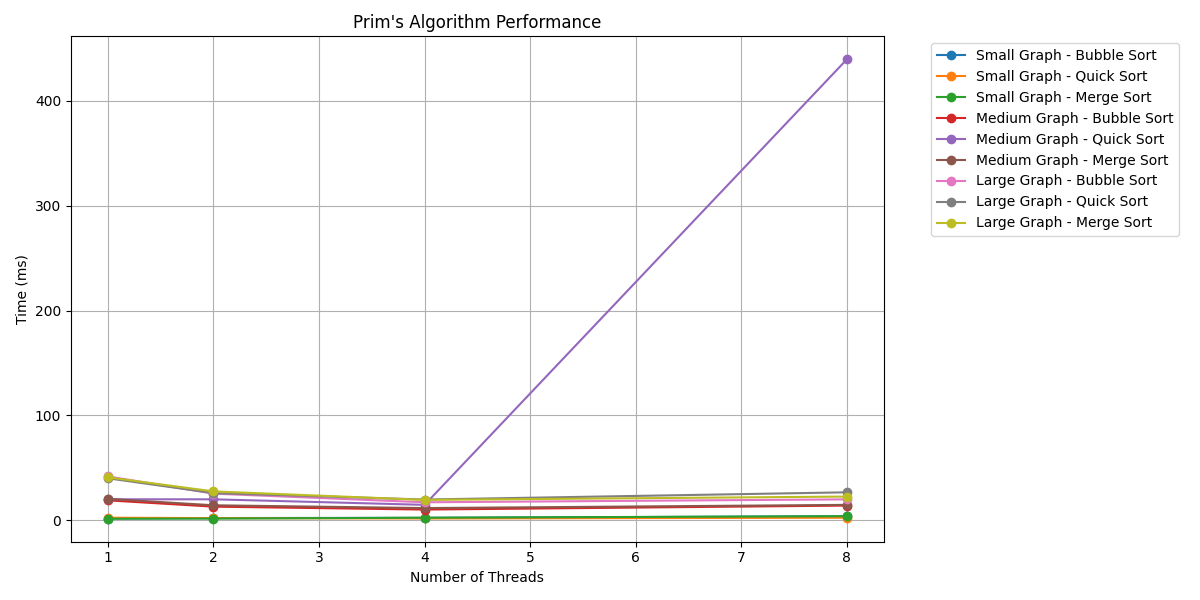
\includegraphics[width=0.8\textwidth]{prims_comparison.png}
    \caption{Prim's Algorithm performance across different graph sizes and sorting methods.}
    \label{fig:prims_comparison}
\end{figure}

\begin{figure}[H]
    \centering
    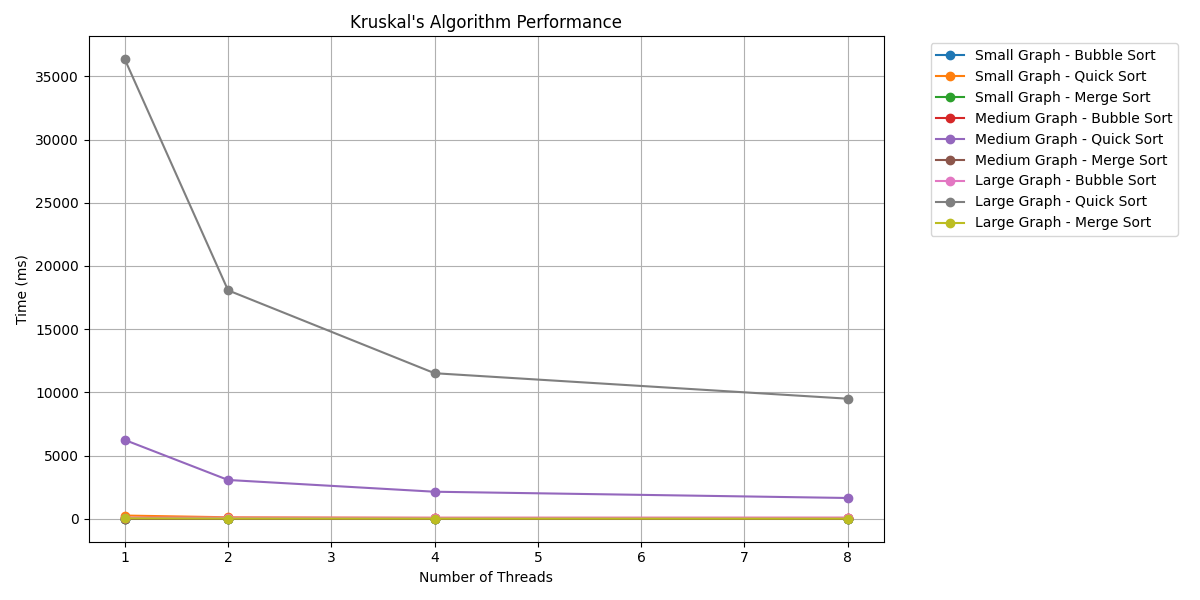
\includegraphics[width=0.8\textwidth]{kruskals_comparison.png}
    \caption{Kruskal's Algorithm performance across different graph sizes and sorting methods.}
    \label{fig:kruskals_comparison}
\end{figure}

\begin{figure}[H]
    \centering
    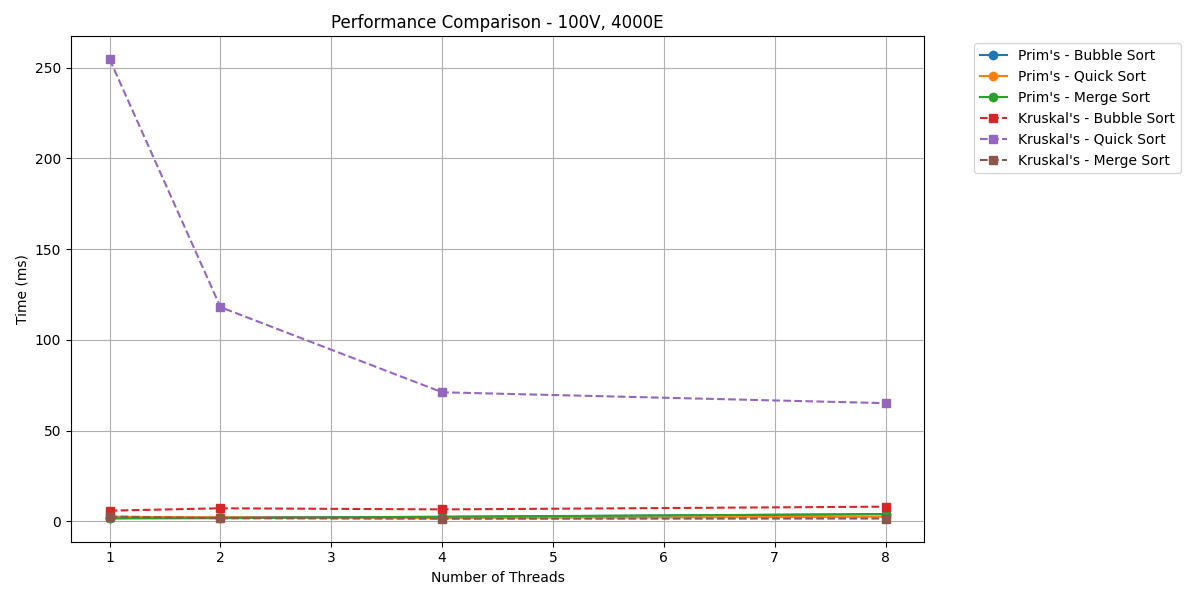
\includegraphics[width=0.8\textwidth]{small_comparison.png}
    \caption{Performance comparison for Small Graph (100V, 4000E).}
    \label{fig:small_comparison}
\end{figure}

\begin{figure}[H]
    \centering
    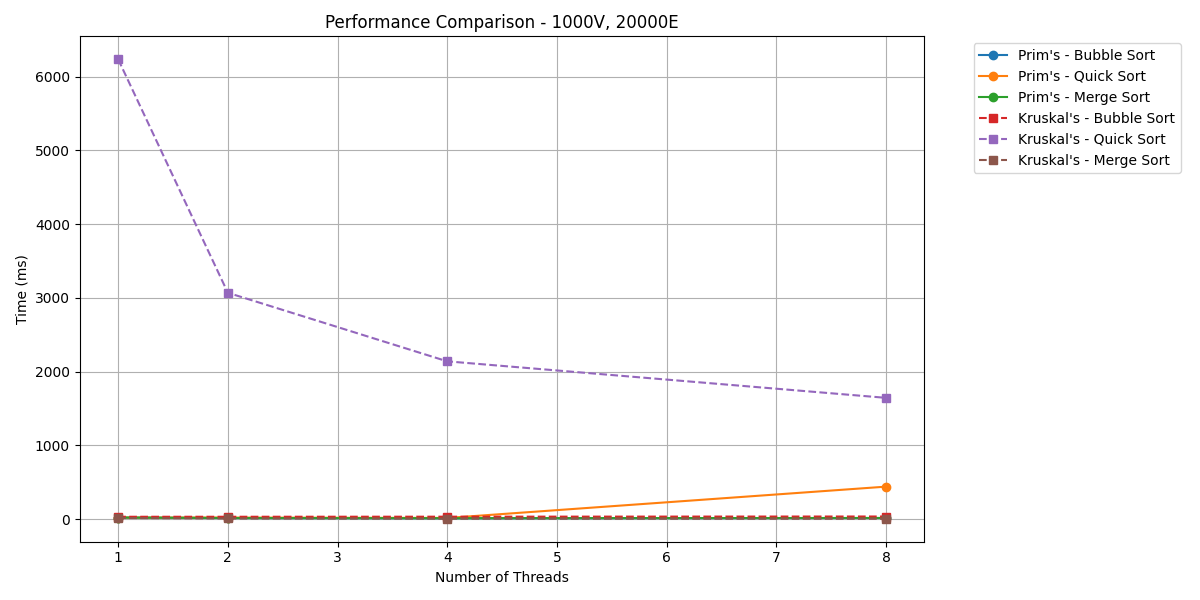
\includegraphics[width=0.8\textwidth]{medium_comparison.png}
    \caption{Performance comparison for Medium Graph (1000V, 20000E).}
    \label{fig:medium_comparison}
\end{figure}

\begin{figure}[H]
    \centering
    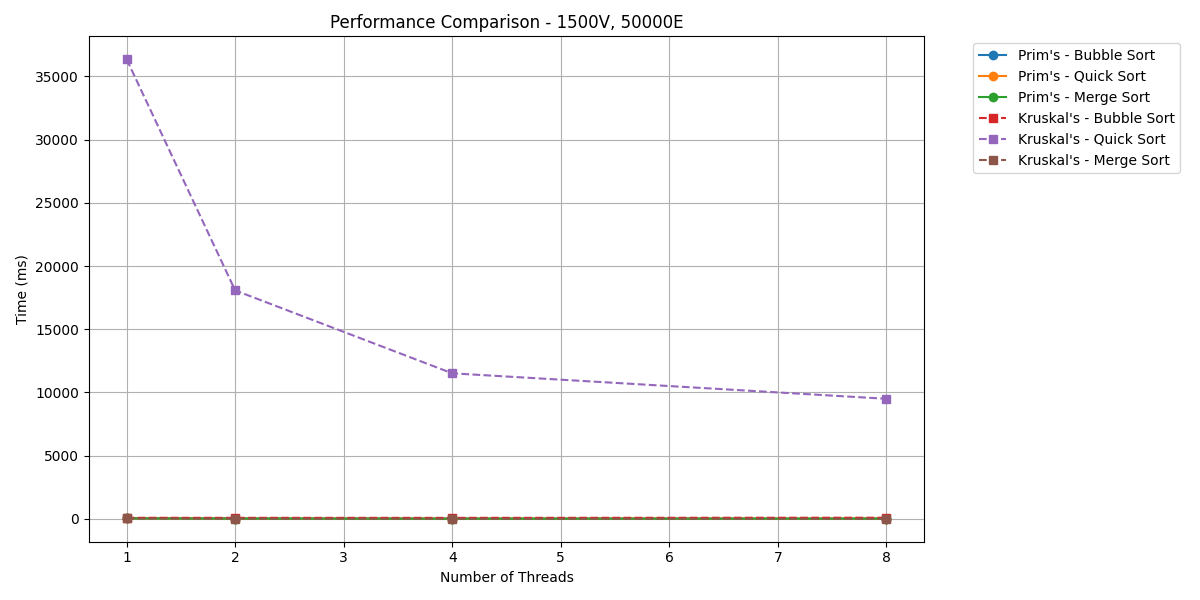
\includegraphics[width=0.8\textwidth]{large_comparison.png}
    \caption{Performance comparison for Large Graph (1500V, 50000E).}
    \label{fig:large_comparison}
\end{figure}

\subsection{Sequential Performance Figures}
\begin{figure}[H]
    \centering
    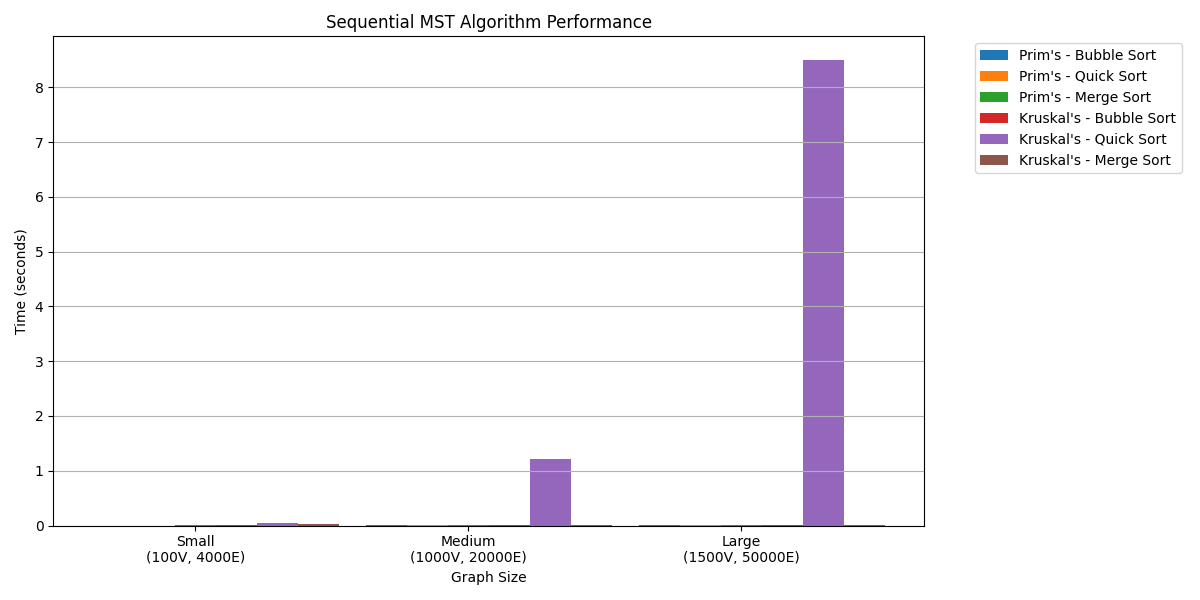
\includegraphics[width=0.8\textwidth]{sequential_comparison.png}
    \caption{Overall sequential performance comparison.}
    \label{fig:sequential_comparison}
\end{figure}

\begin{figure}[H]
    \centering
    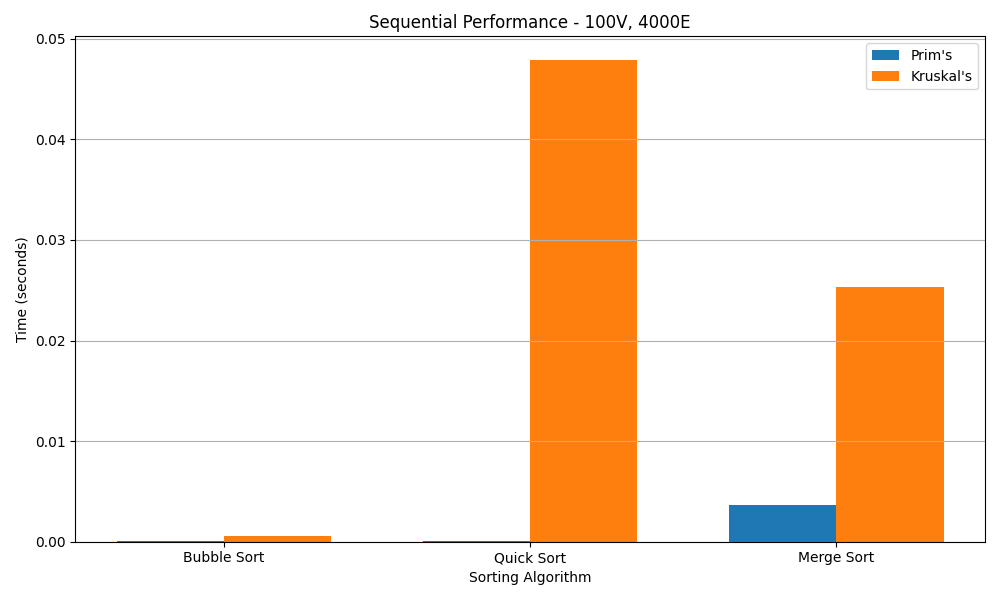
\includegraphics[width=0.8\textwidth]{sequential_small.png}
    \caption{Sequential performance for Small Graph (100V, 4000E).}
    \label{fig:sequential_small}
\end{figure}

\begin{figure}[H]
    \centering
    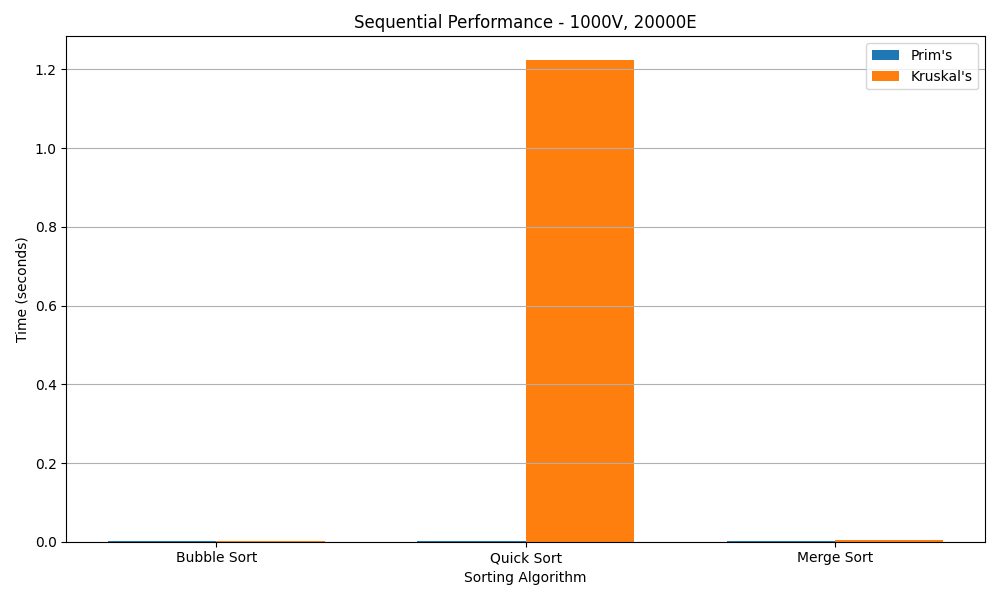
\includegraphics[width=0.8\textwidth]{sequential_medium.png}
    \caption{Sequential performance for Medium Graph (1000V, 20000E).}
    \label{fig:sequential_medium}
\end{figure}

\begin{figure}[H]
    \centering
    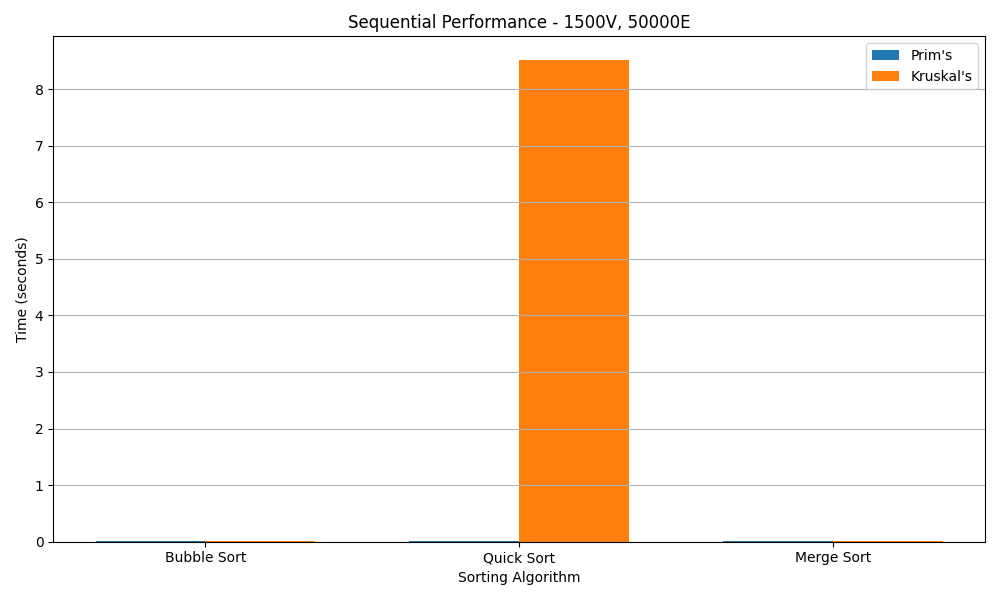
\includegraphics[width=0.8\textwidth]{sequential_large.png}
    \caption{Sequential performance for Large Graph (1500V, 50000E).}
    \label{fig:sequential_large}
\end{figure}

\section{Key Observations and Discussion}
\begin{itemize}
    \item \textbf{Prim's Algorithm:} 
    \begin{itemize}
        \item Scales effectively with increased graph size and thread count.
        \item Exhibits consistent performance with all sorting methods.
        \item Merge Sort often yields the best overall performance.
    \end{itemize}
    \item \textbf{Kruskal's Algorithm:}
    \begin{itemize}
        \item Performance is strongly influenced by the sorting method.
        \item Quick Sort performs poorly for larger graphs, while Merge Sort is most reliable.
        \item Bubble Sort shows limited improvement in parallel configurations.
    \end{itemize}
    \item \textbf{Parallel vs. Sequential:} 
    \begin{itemize}
        \item Significant speedup is observed in parallel implementations for medium and large graphs.
        \item For small graphs, the overhead of parallelization can negate performance gains.
    \end{itemize}
\end{itemize}

\section{Contributing and License}
Contributions to the project are welcome. Please submit pull requests on the GitHub repository:
\begin{center}
\url{https://github.com/Prithviraj8/parallelizing_mst}
\end{center}
This project is licensed under the MIT License; please see the \texttt{LICENSE} file for details.

\section{Conclusion}
This report provides a comprehensive overview of the \textbf{ParallelMST} project. Our work demonstrates that while Prim's algorithm generally outperforms Kruskal's, the choice of sorting method is critical—especially for Kruskal's implementation. The parallel implementations show promising scalability for larger graph instances, offering valuable insights into the trade-offs in parallelizing classic graph algorithms using OpenMP.

\end{document}
